% Member 4 - Section 3.7 Experimental Design and Fair Comparison
\subsection{Experimental Design and Fair Comparison}
\label{sec:exp_design}

\textit{Experiments.} Four experiments answer the four research questions in the Introduction. Experiment 1 trains the Original group and measures the Photo-versus-target gap. Experiment 2 compares Original against +AdaIN. Experiment 3 compares +AdaIN against +Ours with everything else held fixed. Experiment 4 sweeps the style strength $\alpha \in \{0.25, 0.5, 0.75, 1.0\}$ for both augmentation methods, tracing the relation between stylization strength, structure preservation, and cross-domain accuracy. A $\beta$ ablation for the structure-preserving method is planned alongside Experiment 4 (Section~5.3).

\textit{Fairness controls.} Because the compared methods differ only in their training images, the following quantities are fixed across groups:

\begin{itemize}
\item \textit{Same original data:} all groups train on the identical 1{,}349 Photo Training images from Table~\ref{tab:splits}.
\item \textit{Same style pool:} both augmented groups draw style references from one frozen pool of 10 style images, fixed with a content-hash manifest before any training run. The pool holds external paintings that are not part of PACS, and the checker verifies this mechanically (the ``No test-set leakage'' item below).
\item \textit{Same augmentation count:} each augmented group adds exactly one stylized image per original training image (1{,}349 added images).
\item \textit{Same content--style pairing:} the style image paired with each content image is drawn once with a fixed seed and reused by both generators, so the only difference between the two augmented datasets is the stylization algorithm itself.
\item \textit{Same transform pipeline and classifier:} one training script, one transform definition, one ResNet-18 configuration for all groups.
\item \textit{Same optimization budget:} all groups receive the same number of optimizer steps, $S = 660$, computed as 30 passes over the Original training set at batch size 64 ($30 \times 22$). Groups with larger training sets accordingly run fewer passes over their data. Validation is evaluated at the same step cadence for every group.
\item \textit{Same evaluation and seeds:} all groups use the test lists of Table~\ref{tab:splits} and are run with seeds $\{0, 1, 2\}$.
\item \textit{No checkpoint selection:} the reported model is the final checkpoint of the fixed step budget, for every group and every seed. This removes a selection step that we measured to be harmful (Section~\ref{sec:resnet_baseline}).
\item \textit{No test-set leakage:} the style pool is built from external paintings and contains no PACS image. Because Art Painting, Cartoon, and Sketch are the evaluation domains, a style reference drawn from any of them would place the test appearance into the training set. The checker compares the content hash of every style image against the whole local PACS copy and rejects the run if any style image is a PACS image.
\item \textit{Fairness verification.} A checker script validates these constraints mechanically before training: it confirms that the augmented manifests contain the same original images, the same style pool hash, the same augmentation count, that the content--style pairing is identical in both manifests, that no style image is a PACS image, and that the training configuration fingerprint is identical across groups. The configuration fingerprint is recomputed from the full training configuration recorded in each run summary, so a run whose hyper-parameters differ is rejected. A run that fails any check is excluded from results.
\end{itemize}

\textit{Reporting.} Table~\ref{tab:results} shows the result table format used throughout. Entries are mean$\pm$standard deviation over three seeds. Differences between groups are reported per seed, so that a gain which depends on one favorable seed is visible rather than hidden in the average.

\begin{table}[t]
\caption{Result table. Entries are mean$\pm$standard deviation over three training seeds. The Original row is complete (experiment 1); the two augmented rows are pending delivery of the stylization manifests.}
\label{tab:results}
\centering
\scriptsize
\setlength{\tabcolsep}{2.5pt}
\begin{tabular}{@{}lccccc@{}}
\toprule
Training method & Photo & Art & Cartoon & Sketch & Avg \\
\midrule
Original & $99.0\pm0.3$ & $63.2\pm3.7$ & $25.1\pm1.8$ & $31.5\pm4.2$ & $39.9\pm2.7$ \\
+AdaIN   & -- & -- & -- & -- & -- \\
+Ours    & -- & -- & -- & -- & -- \\
\bottomrule
\end{tabular}
\end{table}

Experiment 1 is complete. The Original group reaches $99.0\%$ on Photo Test but only $39.9\%$ averaged over the three unseen domains, so the domain gap is both large and unambiguous. The gap is not uniform: Art Painting, whose appearance is closest to photography, is recognized at $63.2\%$, whereas Cartoon and Sketch, which discard most photographic cues, fall to $25.1\%$ and $31.5\%$. This ordering is the one we would expect from a classifier that relies mainly on photographic texture, and it identifies Cartoon and Sketch as the domains where style augmentation has the most room to help.

\begin{figure}[t]
\centering
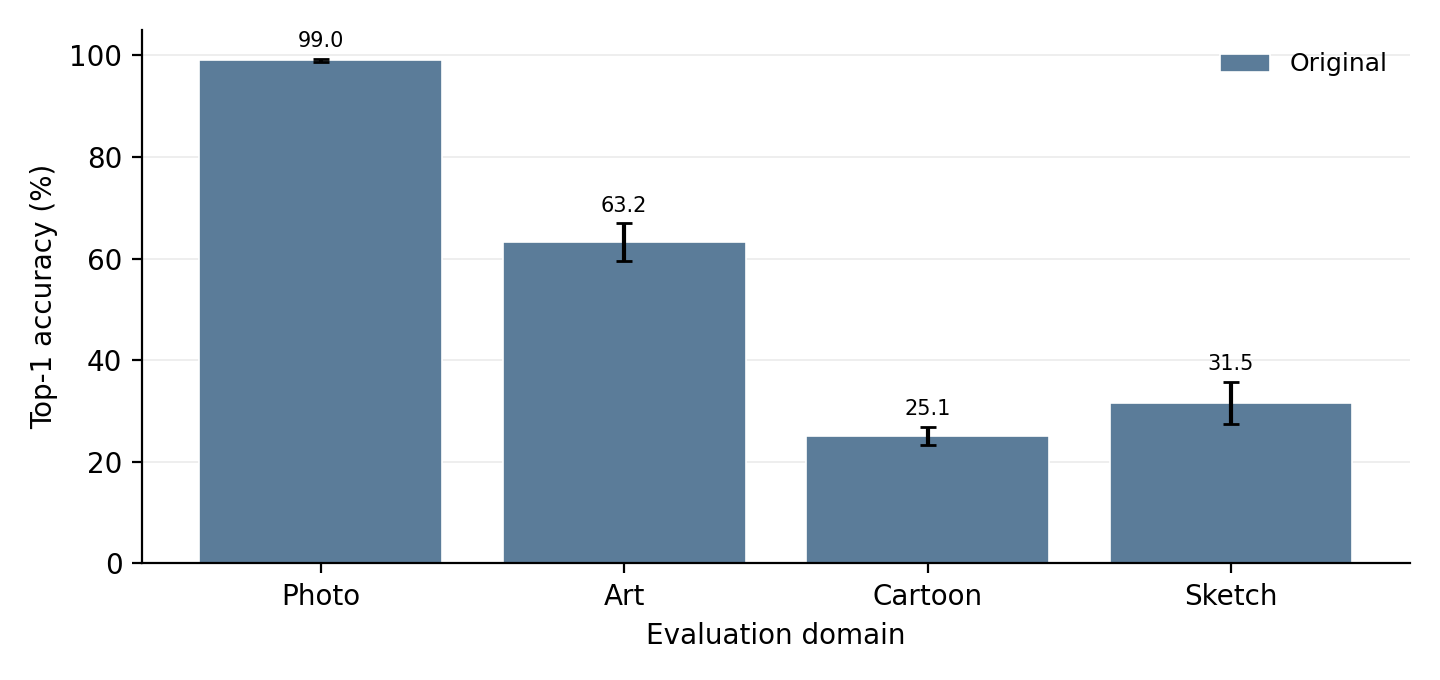
\includegraphics[width=\columnwidth]{figures/results_baseline.png}
\caption{Experiment 1: accuracy of the Original group on the in-domain Photo test set and on the three unseen target domains. Bars are means over three seeds; whiskers are standard deviations.}
\label{fig:results_baseline}
\end{figure}

%==================================================
